\section{Dataset}
In this section, we will describe the custom Khmer traffic sign dataset produced in this project. 
The dataset was manually collected and annotated for traffic sign detection and classification in Cambodia road environments.
\subsection{Dataset Overview}
This paper introduces custom Khmer traffic sign dataset designed for traffic sign detection and classification in Cambodia road conditions.
The proposed dataset was collected and annotated by our team, which consisted of 42 classes that consisting several categories including
regulation, warning, required, and informational signals. The collected images demonstrate various real-world environments with differences
in lighting, angles, distances and backgrounds. Figure 1 demonstrates the complete set of traffic sign classes included in the proposed dataset.
In the next section will detail the data collection, annotation and data statistics.
\begin{figure}[ht]
\fontsize{18}{8}\selectfont 
\begin{center}
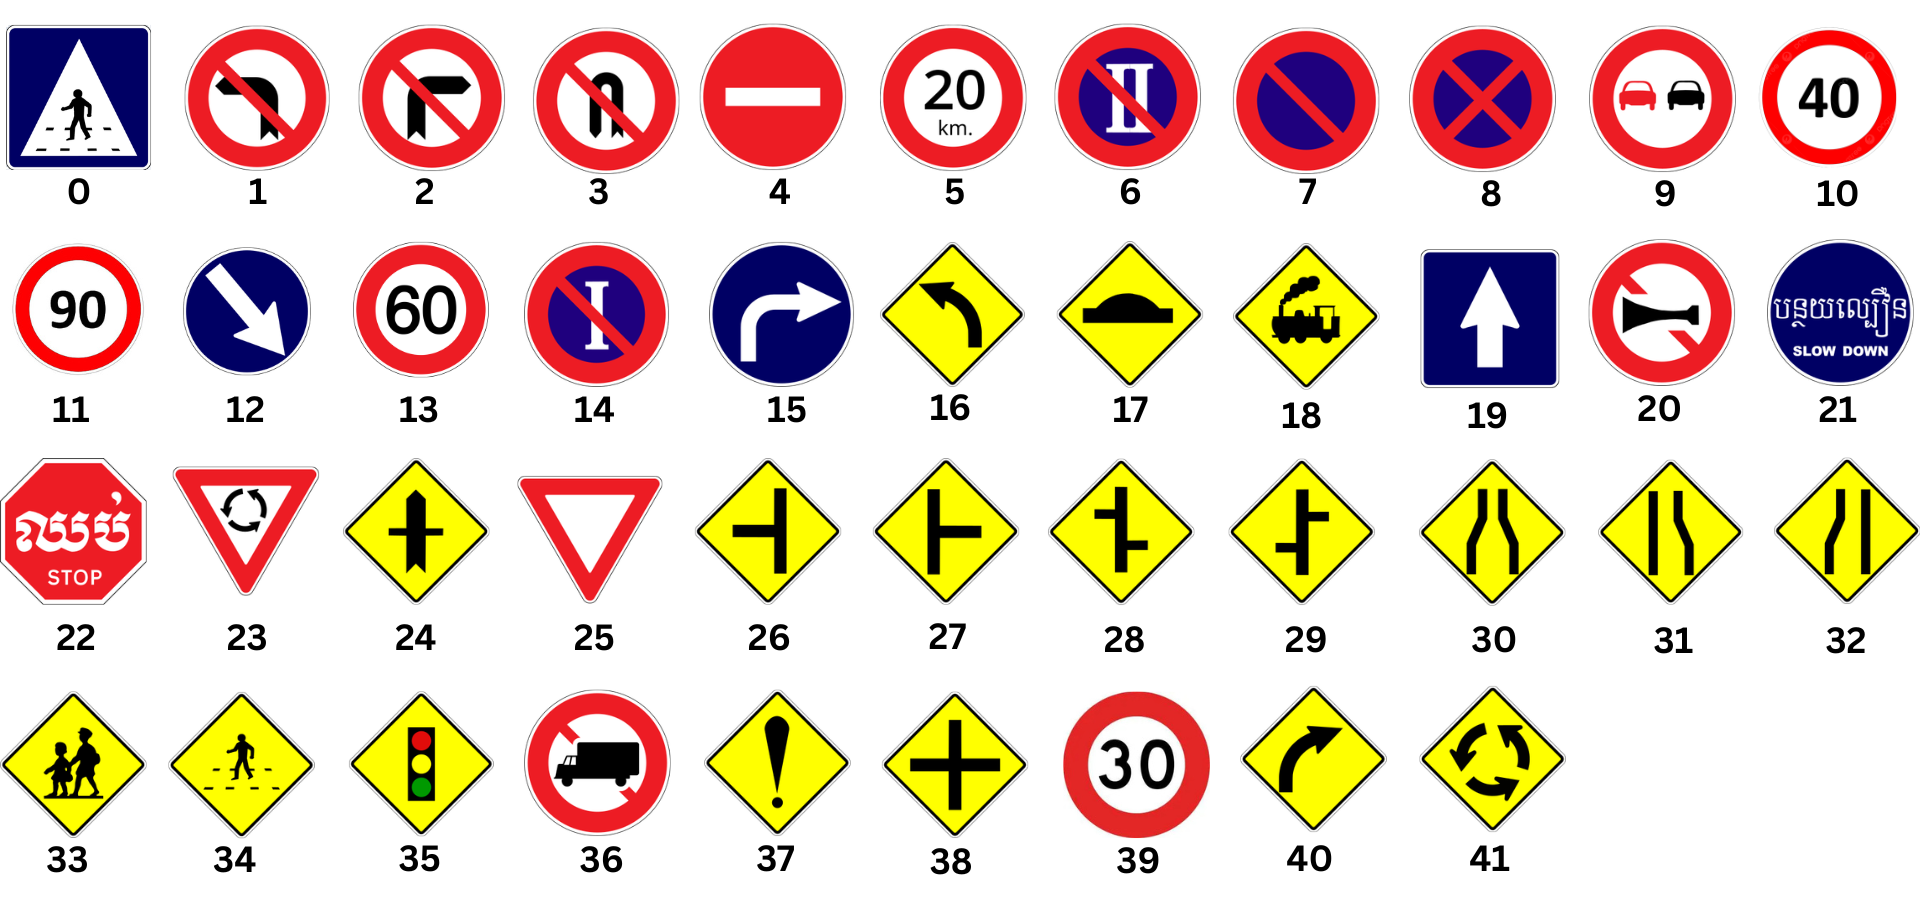
\includegraphics[width=7.4cm]{./fig/Sign_classes.png}
\caption{The 42 traffic sign classes included in the proposed dataset} 
\label{fig:sign_classes}
\end{center}
\end{figure} 
\subsection{Data Collection}
The traffic sign images were manually collected by our team from several sites across Cambodia using a smartphone camera.
Data collecting was conducted on a few different road types, which include urban streets and rural streets. Images were taken under different
real-world conditions, such as different lighting conditions, viewing angles, object distances, and background environments, to boost dataset diversity.
After data gathering, all the images were carefully reviewed to remove duplicate images, images without traffic signs, and images that contain poor visibility that
prevented clear identification of the traffic signs. This process ensured that only the quality images were left for data annotation process.
\subsection{Data Annotation}
Following data collection, all the images were manually annotated using the CVAT annotation tool. Each traffic sign was allocated a rectangular bounding box and
provided with a class label according to one of the 42 predefined traffic sign classes. The annotations were exported in the YOLO format, containing the class
identifier and normalized bounding box coordinates for each signs. To ensure annotations quality, all annotations have been manually validated by our team, and incorrect class labels or inaccurate
bounding boxes were fixed before finish datasets.
\begin{figure}[ht]
    \centering
    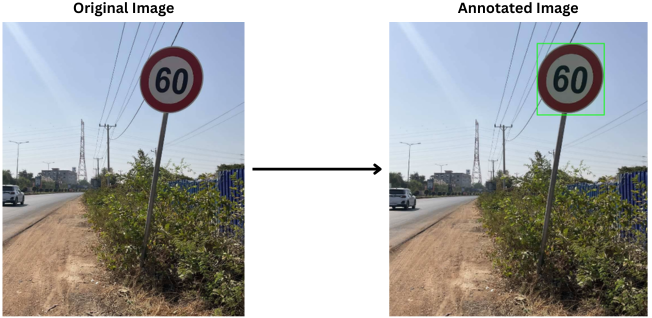
\includegraphics[width=7.4cm]{./fig/Annotated_Image.png}
    \caption{Example of the traffic sign annotation process. Original image. Annotated image with bounding box and class label generated using CVAT}
    \label{fig:annotation}
\end{figure}
\subsection{Data Statistics}